\begin{figure}[htbp]
\centering
\begin{subfigure}{.4\textwidth}
  \centering
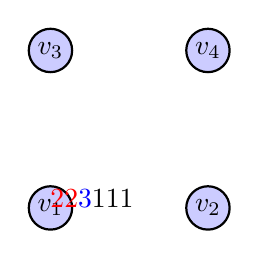
\begin{tikzpicture}[scale=1]
\begin{scope}[every node/.style={circle,thick,draw, inner sep=1.7pt, fill=blue!20}]
    \node (v1) at (0,0) {$v_1$};
    \node (v2) at (2,0) {$v_2$};
    \node (v4) at (2,2) {$v_4$};
    \node (v3) at (0,2) {$v_3$};
\end{scope}
    \Edge[color=red,label=$\color{red}{2}$,style={pos=0.7}](v3)(v2)
    \Edge[color=red,label=$\color{red}{2}$,style={pos=0.5}](v4)(v2)
        \Edge[color=blue,label=$\color{blue}{3}$,style={pos=0.5}](v3)(v4)
\Edge[label=$1$,style={pos=0.7}](v4)(v1)
\Edge[label=$1$,style={pos=0.5}](v1)(v2)
\Edge[label=$1$,style={pos=0.5}](v1)(v3)
\end{tikzpicture}
\end{subfigure}
\begin{subfigure}{.4\textwidth}
  \centering
 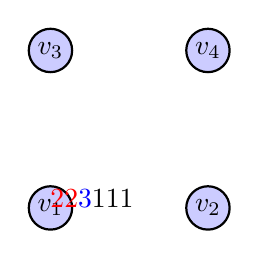
\begin{tikzpicture}[scale=1]
\begin{scope}[every node/.style={circle,thick,draw, inner sep=1.7pt, fill=blue!20}]
    \node (v1) at (0,0) {$v_1$};
    \node (v2) at (2,0) {$v_2$};
    \node (v4) at (2,2) {$v_4$};
    \node (v3) at (0,2) {$v_3$};
\end{scope}
    \Edge[color=red,label=$\color{red}{2}$,style={pos=0.5}](v3)(v1)
    \Edge[color=red,label=$\color{red}{2}$,style={pos=0.5}](v4)(v2)
        \Edge[color=blue,label=$\color{blue}{3}$,style={pos=0.25}](v1)(v4)
\Edge[label=$1$,style={pos=0.5}](v4)(v3)
\Edge[label=$1$,style={pos=0.5}](v1)(v2)
\Edge[label=$1$,style={pos=0.25}](v2)(v3)
\end{tikzpicture}
\end{subfigure}
\caption{Two nonisomorphic MAT-labelings of $K_4$ constructed by using Lemma \ref{MAT-L-PEO of complete graph}\ref{MAT-L-PEO of complete graph 2} (left) and the ideal MAT-free theorem (right).}
\label{fig:MAT-K4}
\end{figure}
